\documentclass{../tuda-beamer}

% Title information
\authors{Nhan Huynh}
\authors{Daniel Mangold}
\date{27. Oktober 2021}

\begin{document}

    \maketitle

    \begin{frame}{Überblick}
        \tableofcontents
    \end{frame}


    \section{Organisatorisches}
    \begin{frame}[c]
        \begin{center}
            \textbf{\LARGE Vorstellung}
        \end{center}
    \end{frame}

    \begin{frame}{Organisatorisches}
        \begin{itemize}
            \item Mittwoch 16:45 - 18:25
            \item S103/123 (vereinzelt Raumabweichung - siehe Moodle)
            \item Klausurzulassung: Studienleistung
            \begin{itemize}
                \item 50\% der Gesamtpunktzahl der Hausübungen
                \item Frühzeitig anfangen, da spätere Hausübungen komplexer werden!
            \end{itemize}
            \item Bonus: Jeder weitere Punkt über die 50\% der Gesamtpunktzahl der Hausübungen wird
            mittels einer Formel in Klausurpunkte umgerechnet
            \item Projekt: Infos ca. rund um Weihnachten
        \end{itemize}
    \end{frame}

    \begin{frame}{Hinweise}
        \begin{itemize}
            \item FAQ zu jeder Hausübung
            \item Moodle Forum
            \item Discord bzw. Sprechstunden
            \item Themensprechstunde
            \begin{itemize}
                \item Mittwoch 14:30 - 16:30
                \item Präsenz \& Livestream
            \end{itemize}
            \item Check + Prepare Kurs
            \begin{itemize}
                \item Zusätzliches Übungsmaterial
                \item Thematische Zusammenfassung
                \item und vieles mehr!
            \end{itemize}
        \end{itemize}
    \end{frame}

    \begin{frame}[c]
        \begin{figure}[h]
            \centering
            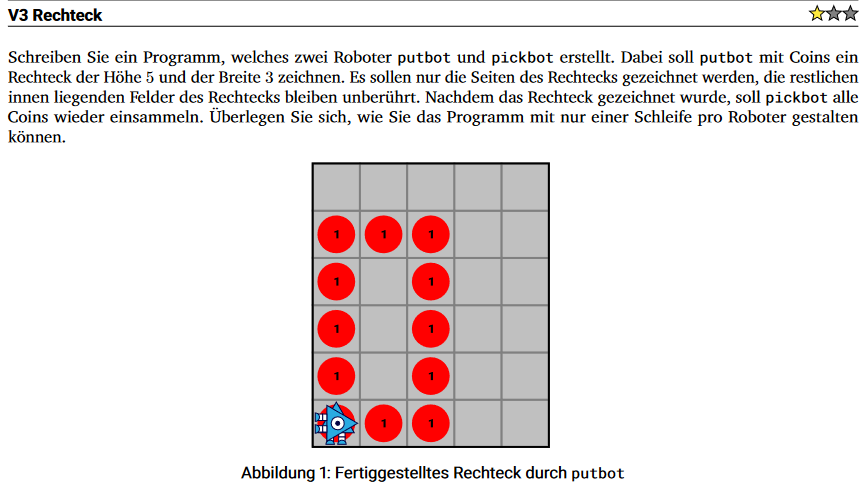
\includegraphics[width=.7\linewidth]{graphics/cp_exercise_example.png}
            \caption{Übungsblatt 01 - V3}
        \end{figure}
    \end{frame}

    \begin{frame}[c]
        \begin{figure}[h]
            \centering
            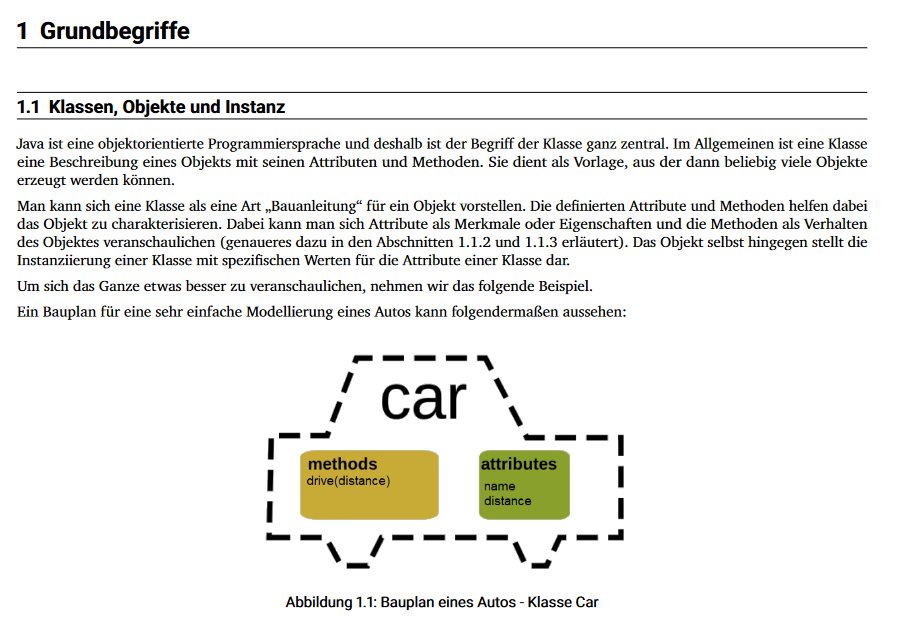
\includegraphics[width=.6\linewidth]{graphics/cp_summary_example.png}
            \caption{Thematische Zusammenfassung Fortgeschritten - Java}
        \end{figure}
    \end{frame}

    \begin{frame}[c]
        \begin{figure}[h]
            \centering
            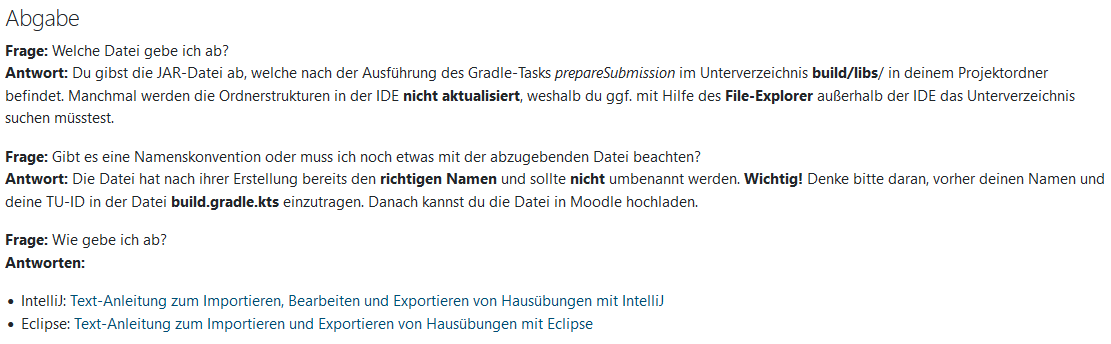
\includegraphics[width=.985\linewidth]{graphics/faq_example.png}
            \caption{FAQ zur Hausübung 0}
        \end{figure}
    \end{frame}


    \section{WLAN-Einrichtung (eduroam)}
    \begin{frame}{WLAN-Einrichtung (eduroam)}
        \begin{itemize}
            \item WLAN: eduroam
            \item \small \url{https://www.hrz.tu-darmstadt.de/services/it_services/wlan/index.de.jsp}
            \item PC
            \begin{itemize}
                \item Anonyme/Äußere Identität: eduroam@tu-darmstadt.de
                \item Benutzerkennung: <tu-id>@tu-darmstadt.de
                \item Passwort: <pw> (selbes wie in Moodle)
            \end{itemize}
            \item Handy
            \begin{itemize}
                \item Automatisch; Configuration Assitant Tool (CAT)
                \item Manuell: Zertifikat T-TeleSec GlobalRoot Class 2
            \end{itemize}
        \end{itemize}
    \end{frame}


    \section{Installation Java}
    \begin{frame}{Installation Java}
        \begin{figure}[h]
            \centering
            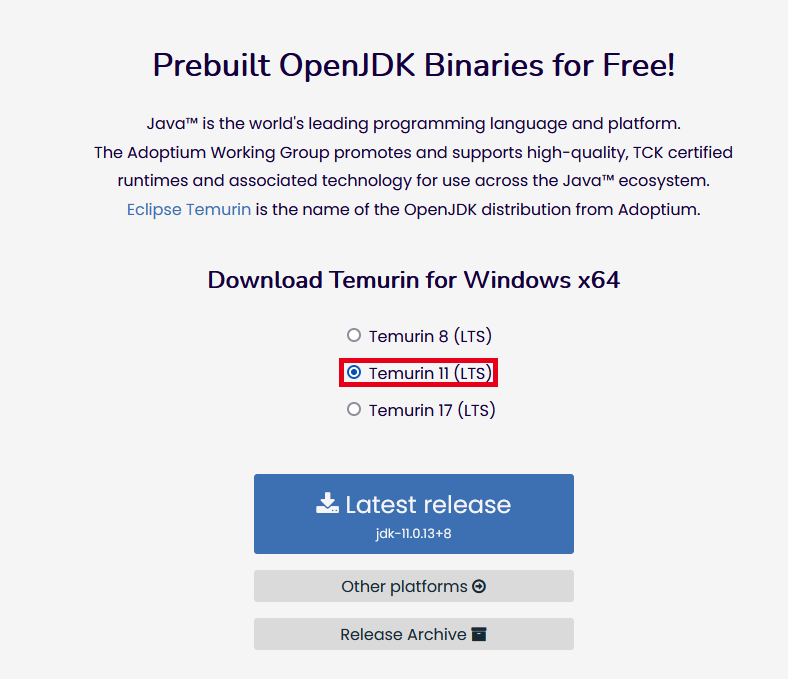
\includegraphics[width=.35\linewidth]{graphics/temurin_11.png}
            \caption{Adoptium - Temurin 11 \url{https://adoptium.net/}}
        \end{figure}
    \end{frame}

    \begin{frame}[c]
        \begin{figure}[h]
            \centering
            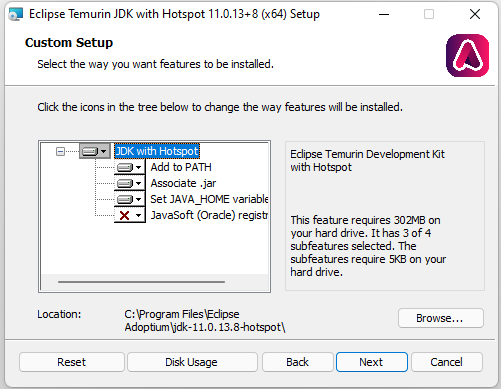
\includegraphics[width=.3\linewidth]{graphics/temurin_installer.png}
            \caption{Temurin Installer}
        \end{figure}
    \end{frame}


    \section{Importieren von Hausübungen}
    \begin{frame}[c]{Importieren von Hausübungen}
        \begin{center}
            \textbf{\LARGE Live}
        \end{center}
    \end{frame}


    \section{Arbeitsphase}
    \begin{frame}[c]{Arbeitsphase}
        \begin{center}
            \textbf{\LARGE Selbstständiges Arbeiten}
        \end{center}
    \end{frame}
\end{document}
